\begin{frame}
\frametitle{Aircraft W\&B}
\begin{center}
Fixed-wing Aircraft Weight and Balance
\end{center}
\end{frame}

\begin{frame}
\frametitle{Fixed-wing Aircraft Weight and Balance}
\begin{block}{Basic principles}
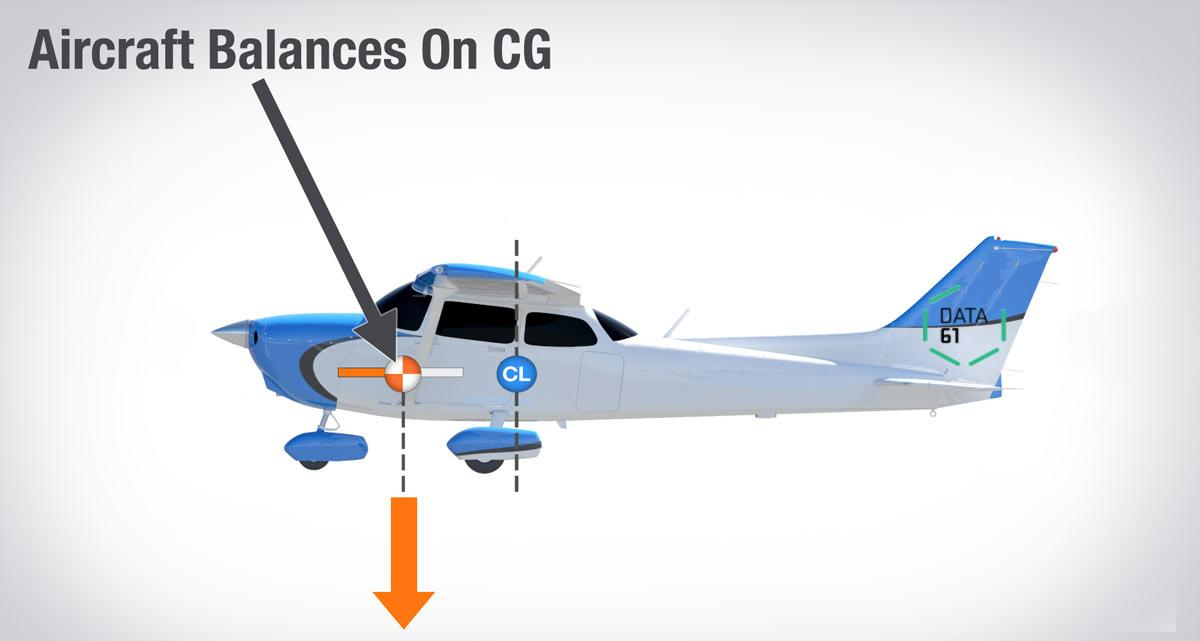
\includegraphics[height=0.5\textheight]{image/aircraft-cg.jpg}
\end{block}
\end{frame}

\begin{frame}
\frametitle{Fixed-wing Aircraft Weight and Balance}
\begin{block}{Same principles apply to A380}
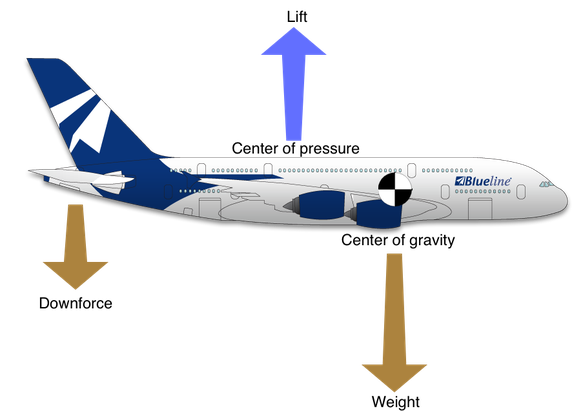
\includegraphics[height=0.5\textheight]{image/aircraft-cg-a380.png}
\end{block}
\end{frame}

\begin{frame}
\frametitle{Fixed-wing Aircraft Weight and Balance}
\begin{block}{Weight}
\begin{itemize}
\item Weight is (loosely) ensuring that the aircraft is not too heavy to maintain flight.
\item Balance is (loosely) ensuring that the CG is positioned such that the aircraft is controllable.
\end{itemize}
\end{block}
\end{frame}

% being under time pressure when a variable changes
